
\documentclass{article}

\usepackage{graphicx}
\usepackage{listings}
\usepackage{color}
\usepackage[a4paper, total={7in, 9in}]{geometry}
\usepackage[section]{placeins}
\usepackage{comment}

\graphicspath{ {./images/} }

\definecolor{dkgreen}{rgb}{0,0.6,0}
\definecolor{gray}{rgb}{0.5,0.5,0.5}
\definecolor{mauve}{rgb}{0.58,0,0.82}

\lstset{frame=tb,
  language=Python,
  aboveskip=3mm,
  belowskip=3mm,
  showstringspaces=false,
  columns=flexible,
  basicstyle={\small\ttfamily},
  numbers=none,
  numberstyle=\tiny\color{gray},
  keywordstyle=\color{blue},
  commentstyle=\color{dkgreen},
  stringstyle=\color{mauve},
  breaklines=true,
  breakatwhitespace=true,
  tabsize=3
}


\title{Protokollierung einer seriellen Schnittstelle auf Basis eines RaspberryPi 4}
\author{Samuel Brunner}

\begin{document}
\maketitle

\section{Funktionsumfang}
Dieses System dient zur Protokollierung einer seriellen RS232 Ausgabeschnittstelle. 
Logfiles werden dabei automatisch auf einen USB-Stick mit Timestamp gesichert. 
Um eine unterbrechungsfreie, zuverlässige und autarke Funktion zu gewährleisten wird eine Powerbank als USV vorgeschalten. Es können Einwegschnittstellen, wie z.B. Debugausgabeports, aber auch Kommunikation zwischen Systemen, ohne diese zu beeinflussen, mitgeschnitten werden.


\section{Hardwarevorbereitung}
\begin{figure}[h]
\caption{Gesamtansicht}
  \centering
    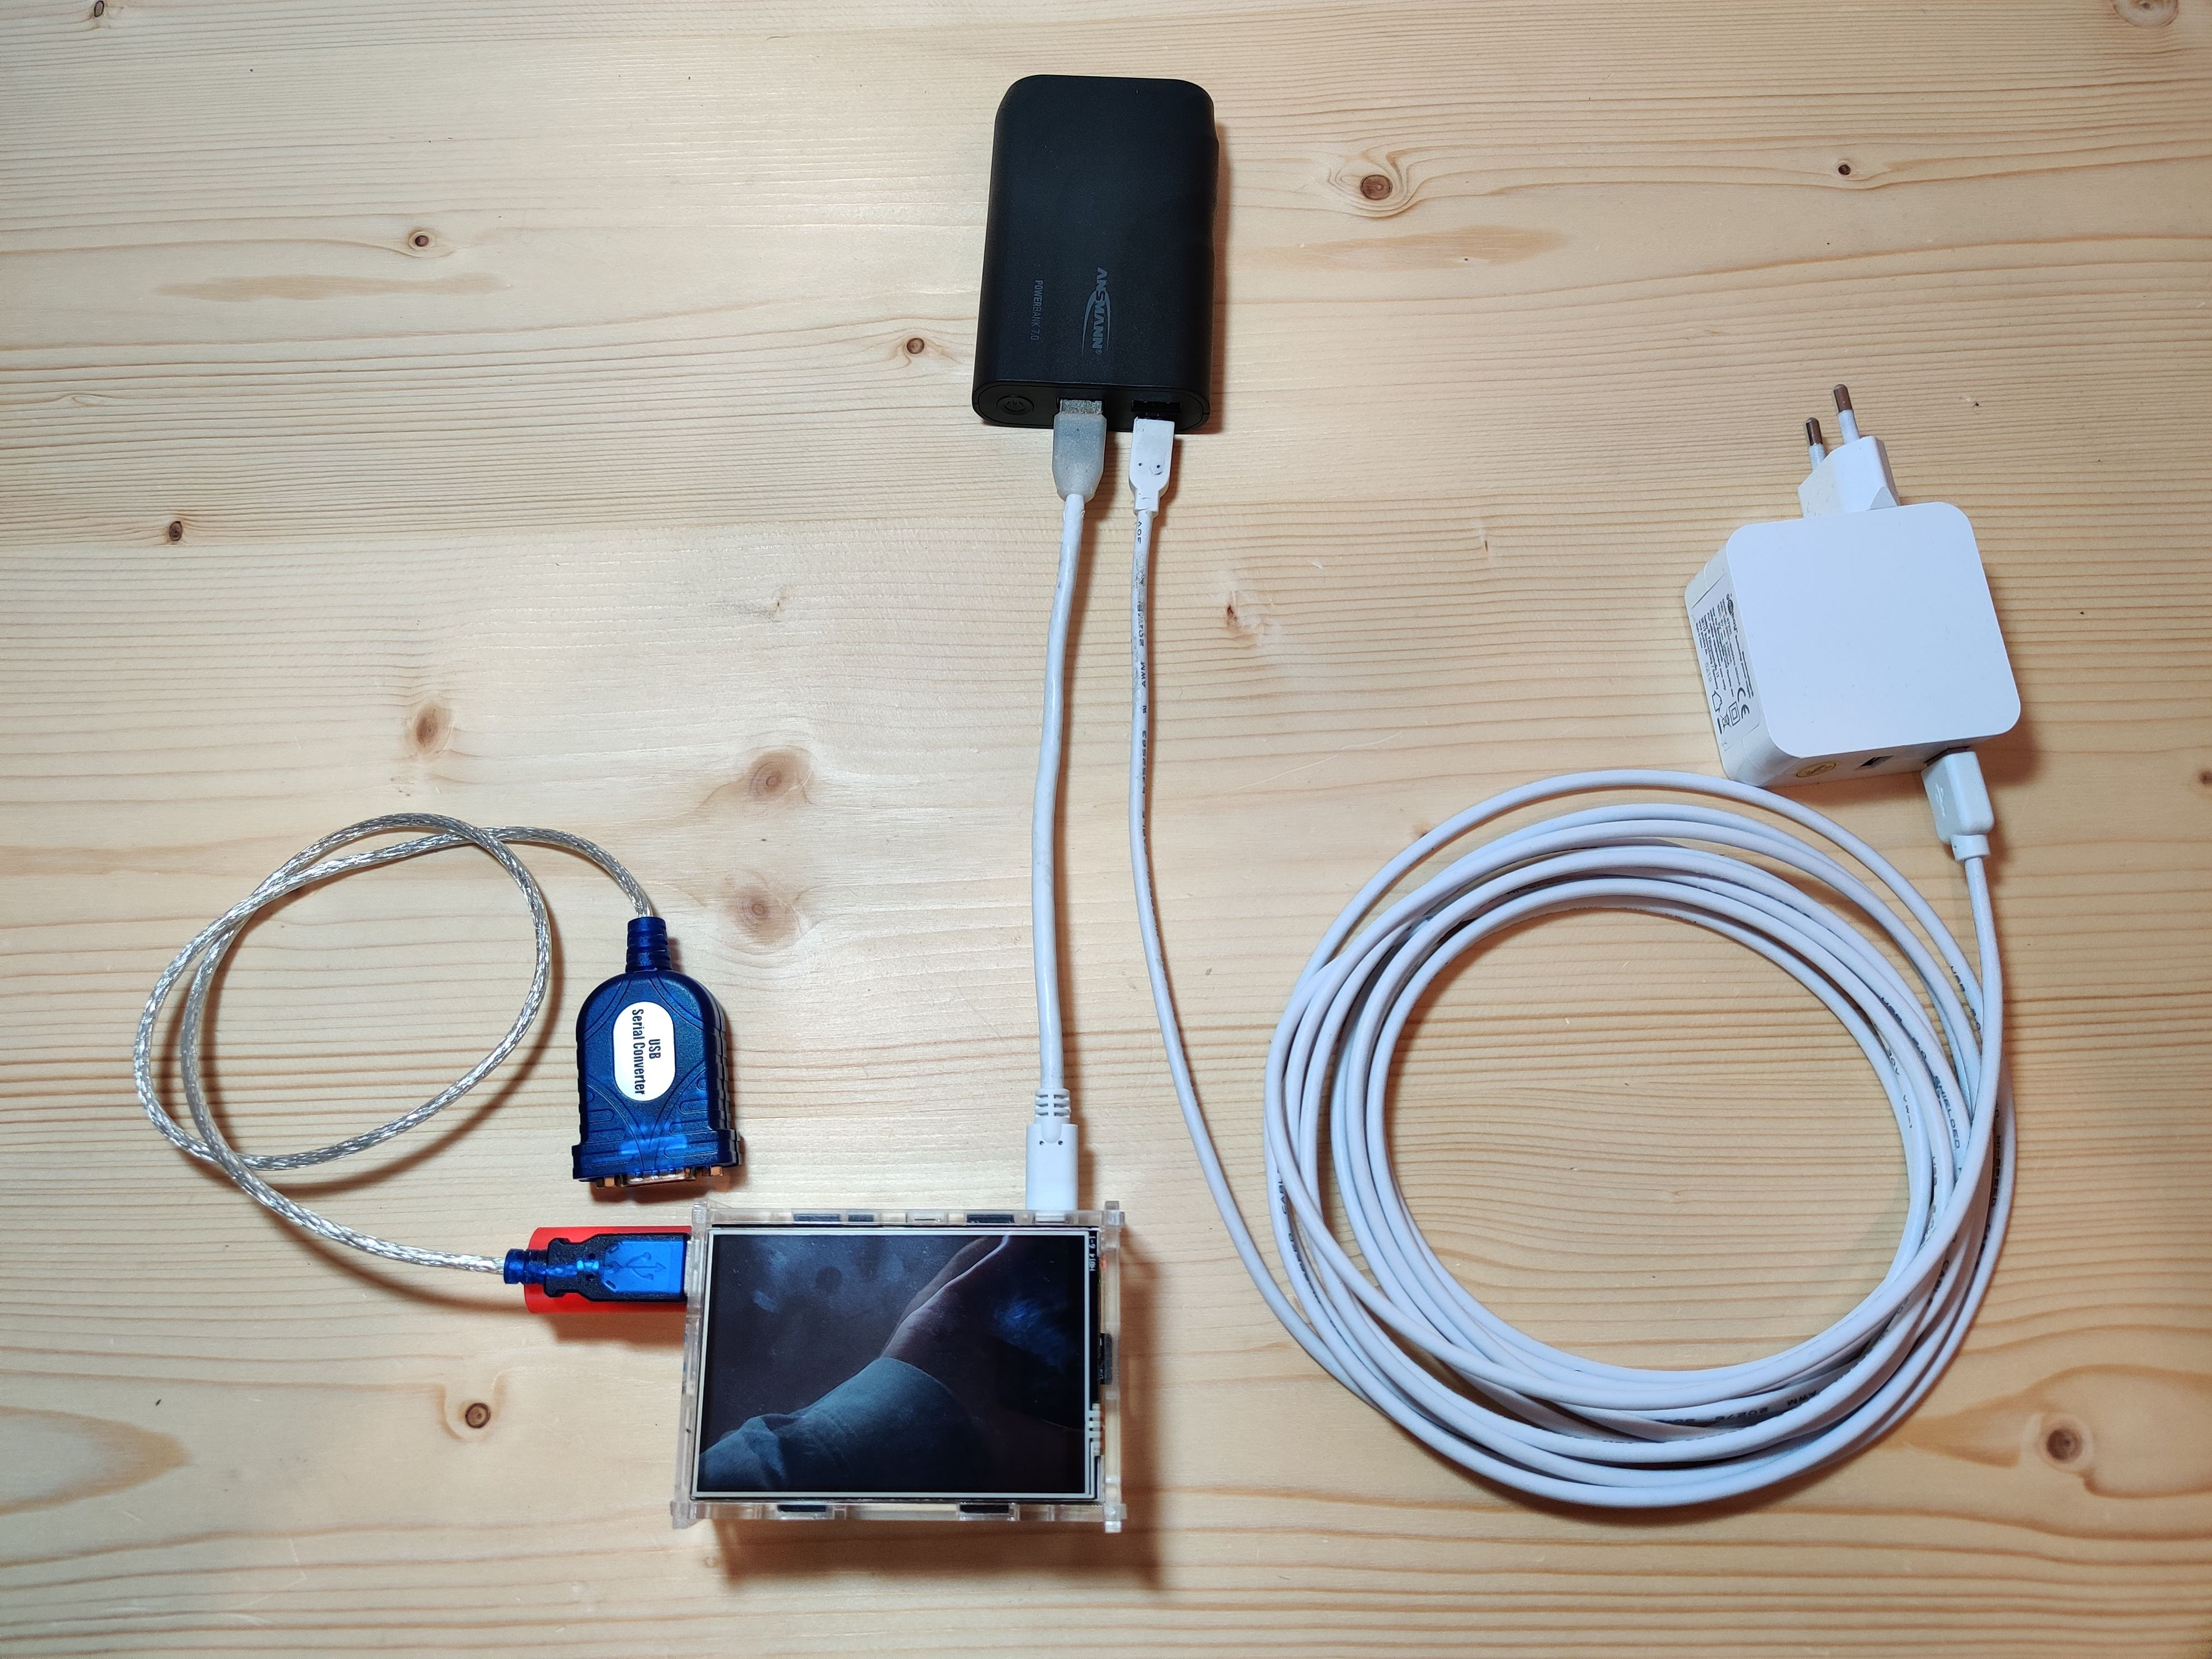
\includegraphics[height=0.5\textheight]{hardware1.jpg}
\end{figure}
\begin{figure}
  \caption{Da muass no de richtige Powerbank nei! De hat koa pass-through-charging}
  \centering
    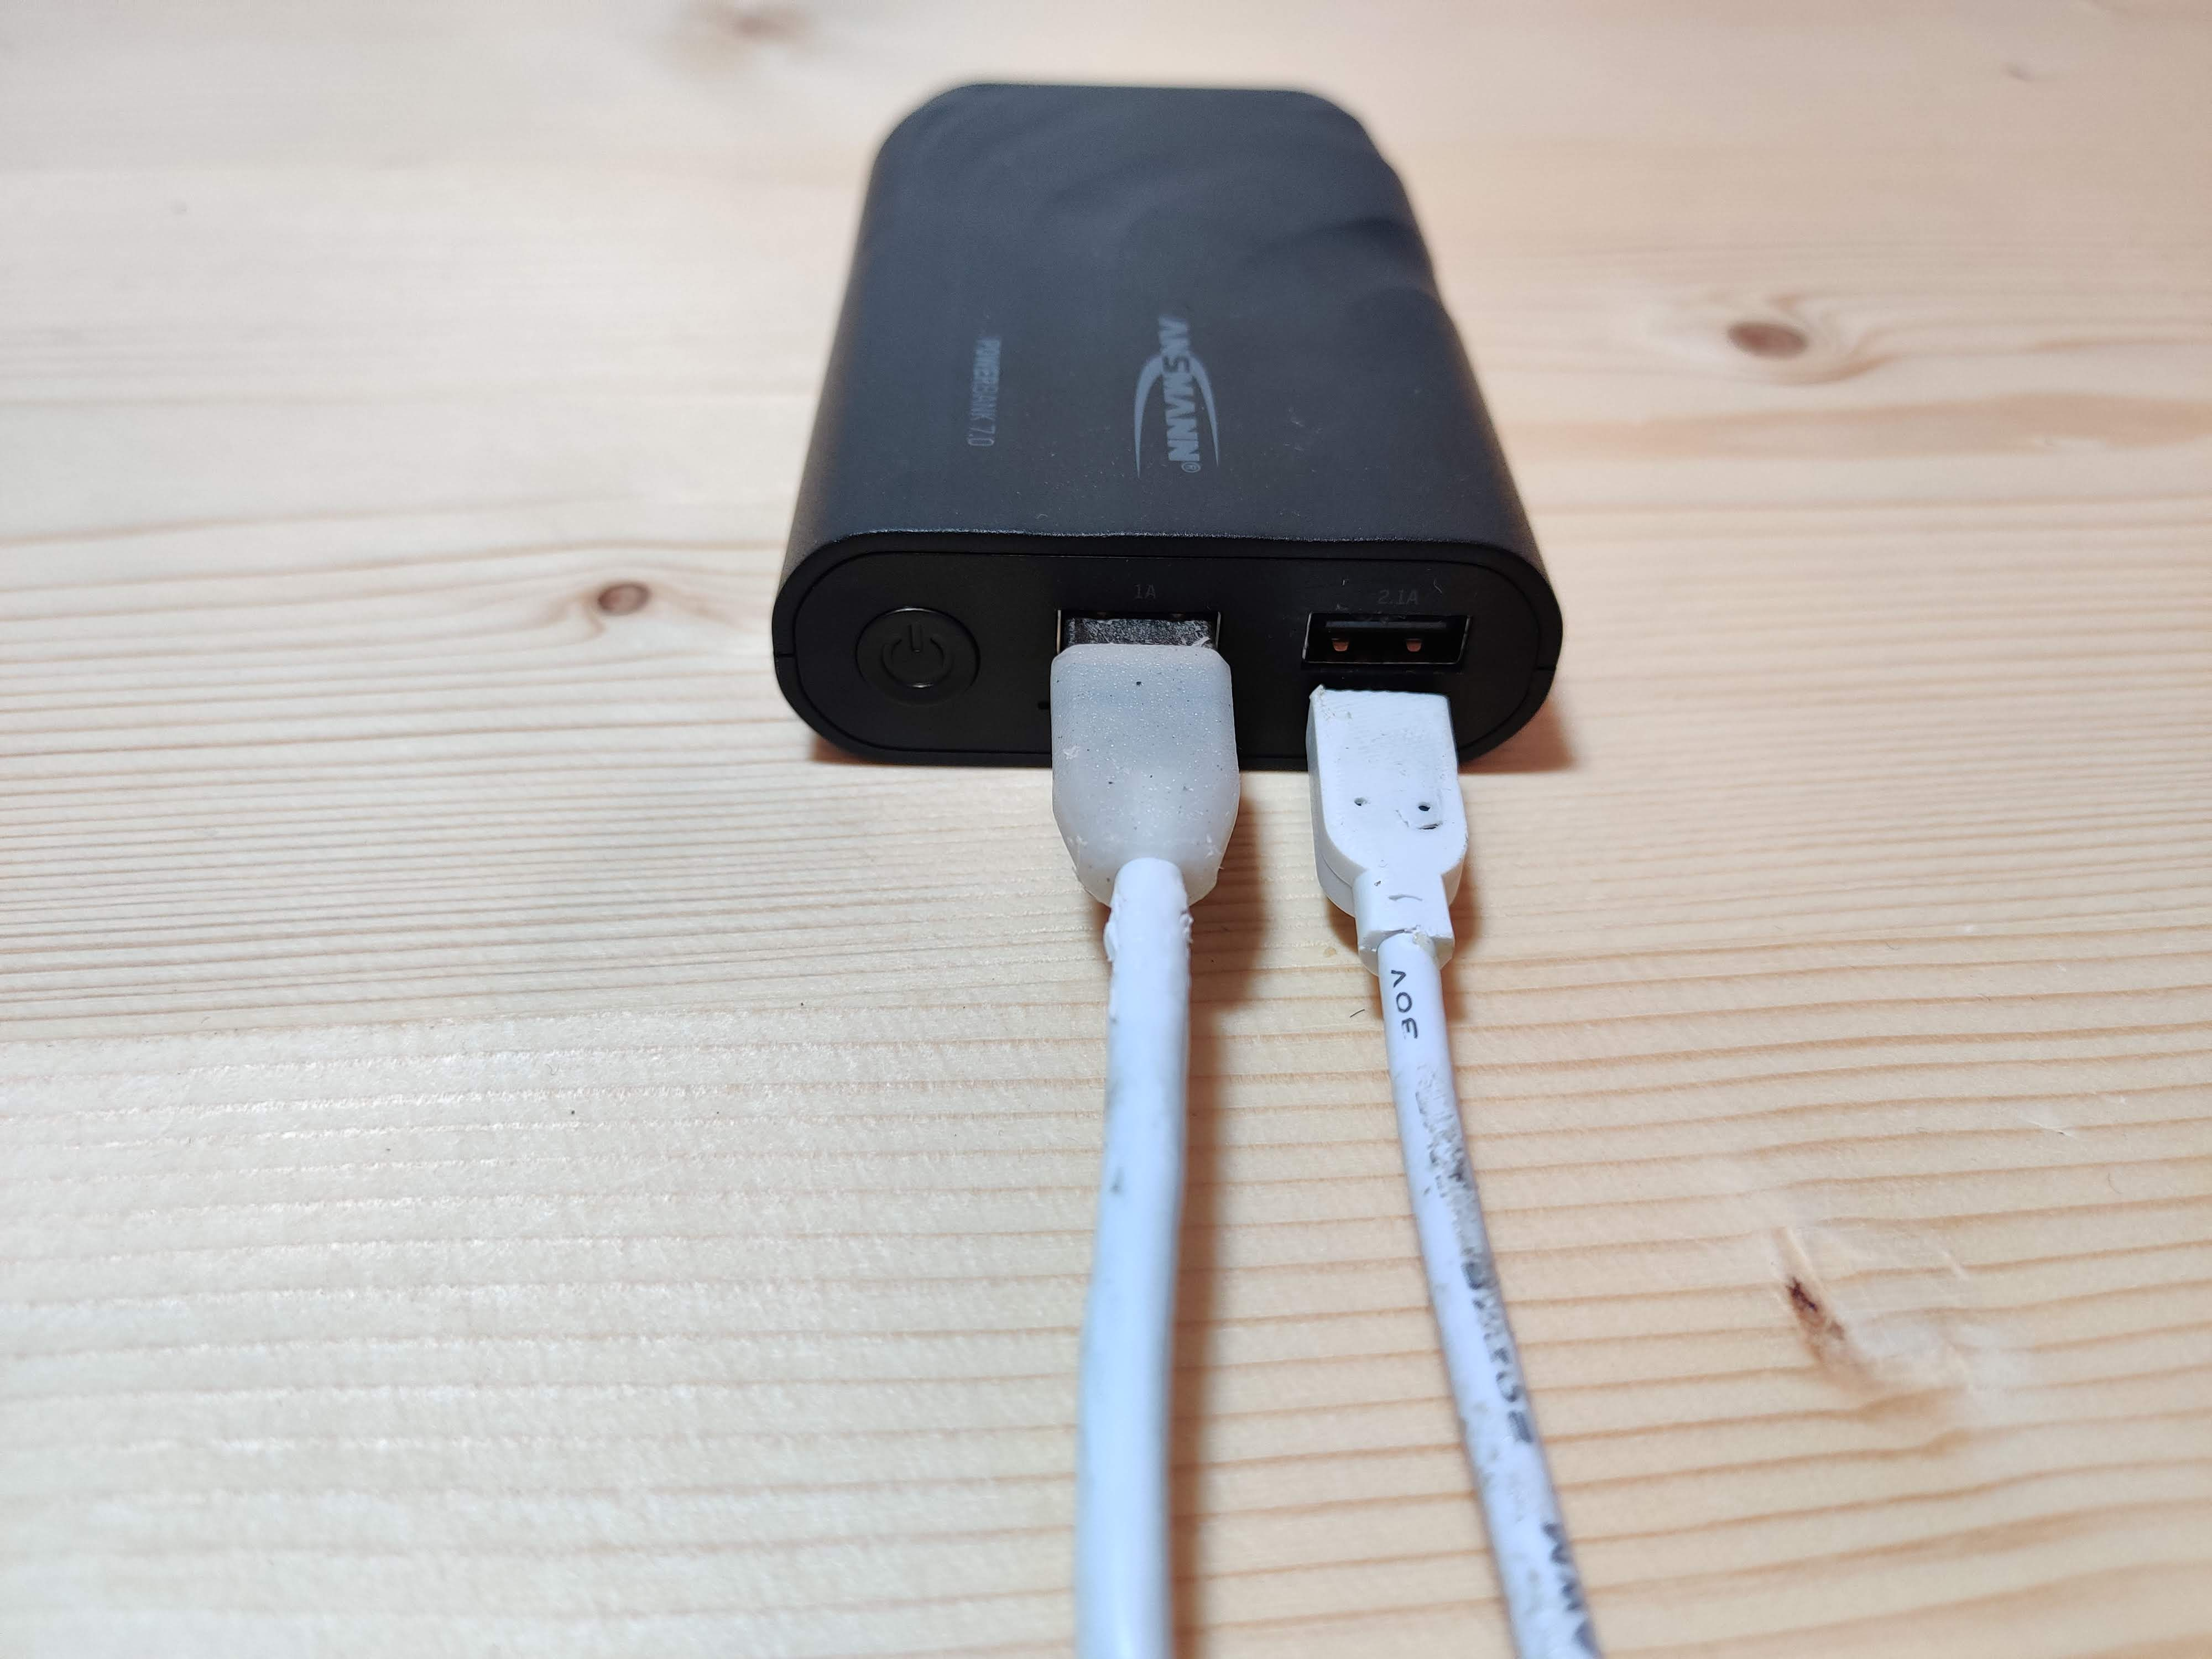
\includegraphics[width=1\textwidth]{hardware2.jpg}
\end{figure}
\begin{figure}
  \caption{USB-RS232-Adapter und USB-Stick an beliebige USB-Ports anstecken}
  \centering
    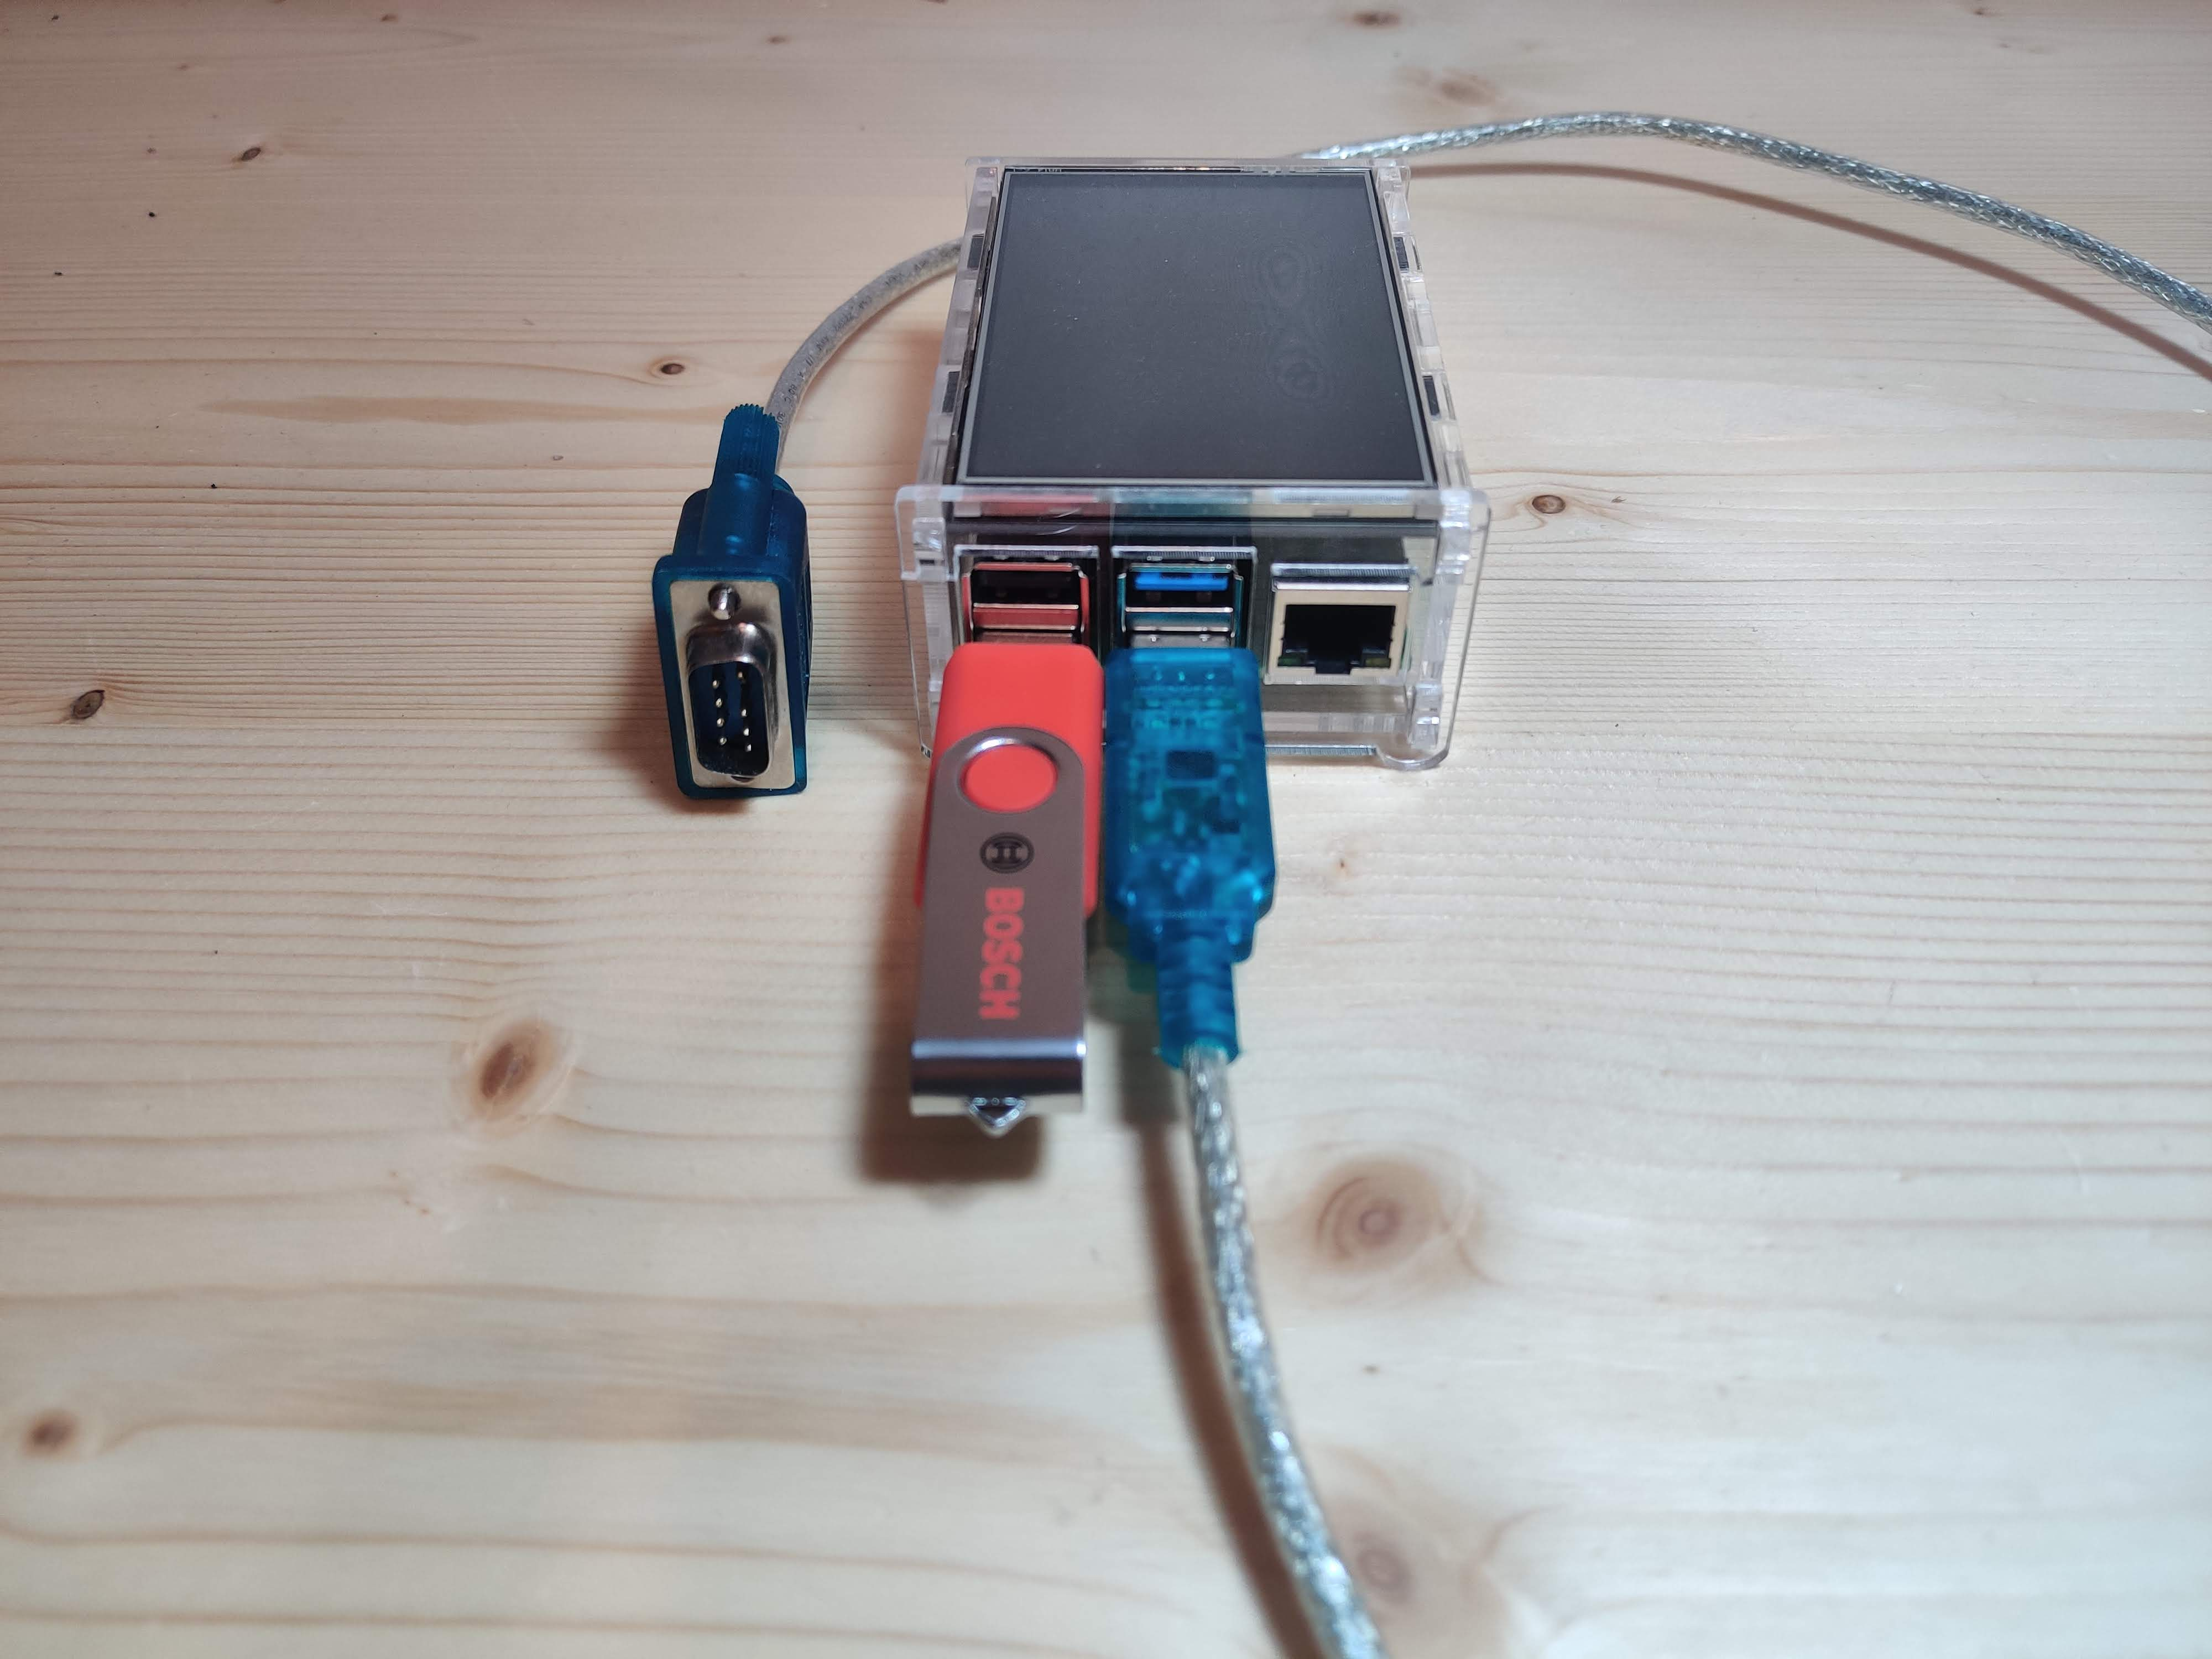
\includegraphics[width=1\textwidth]{hardware3.jpg}
\end{figure}
\begin{figure}
  \caption{Nur für bidirektionales logging: Zwei USB-RS232-Adapter und USB-Stick an beliebige USB-Ports anstecken}
  \centering
    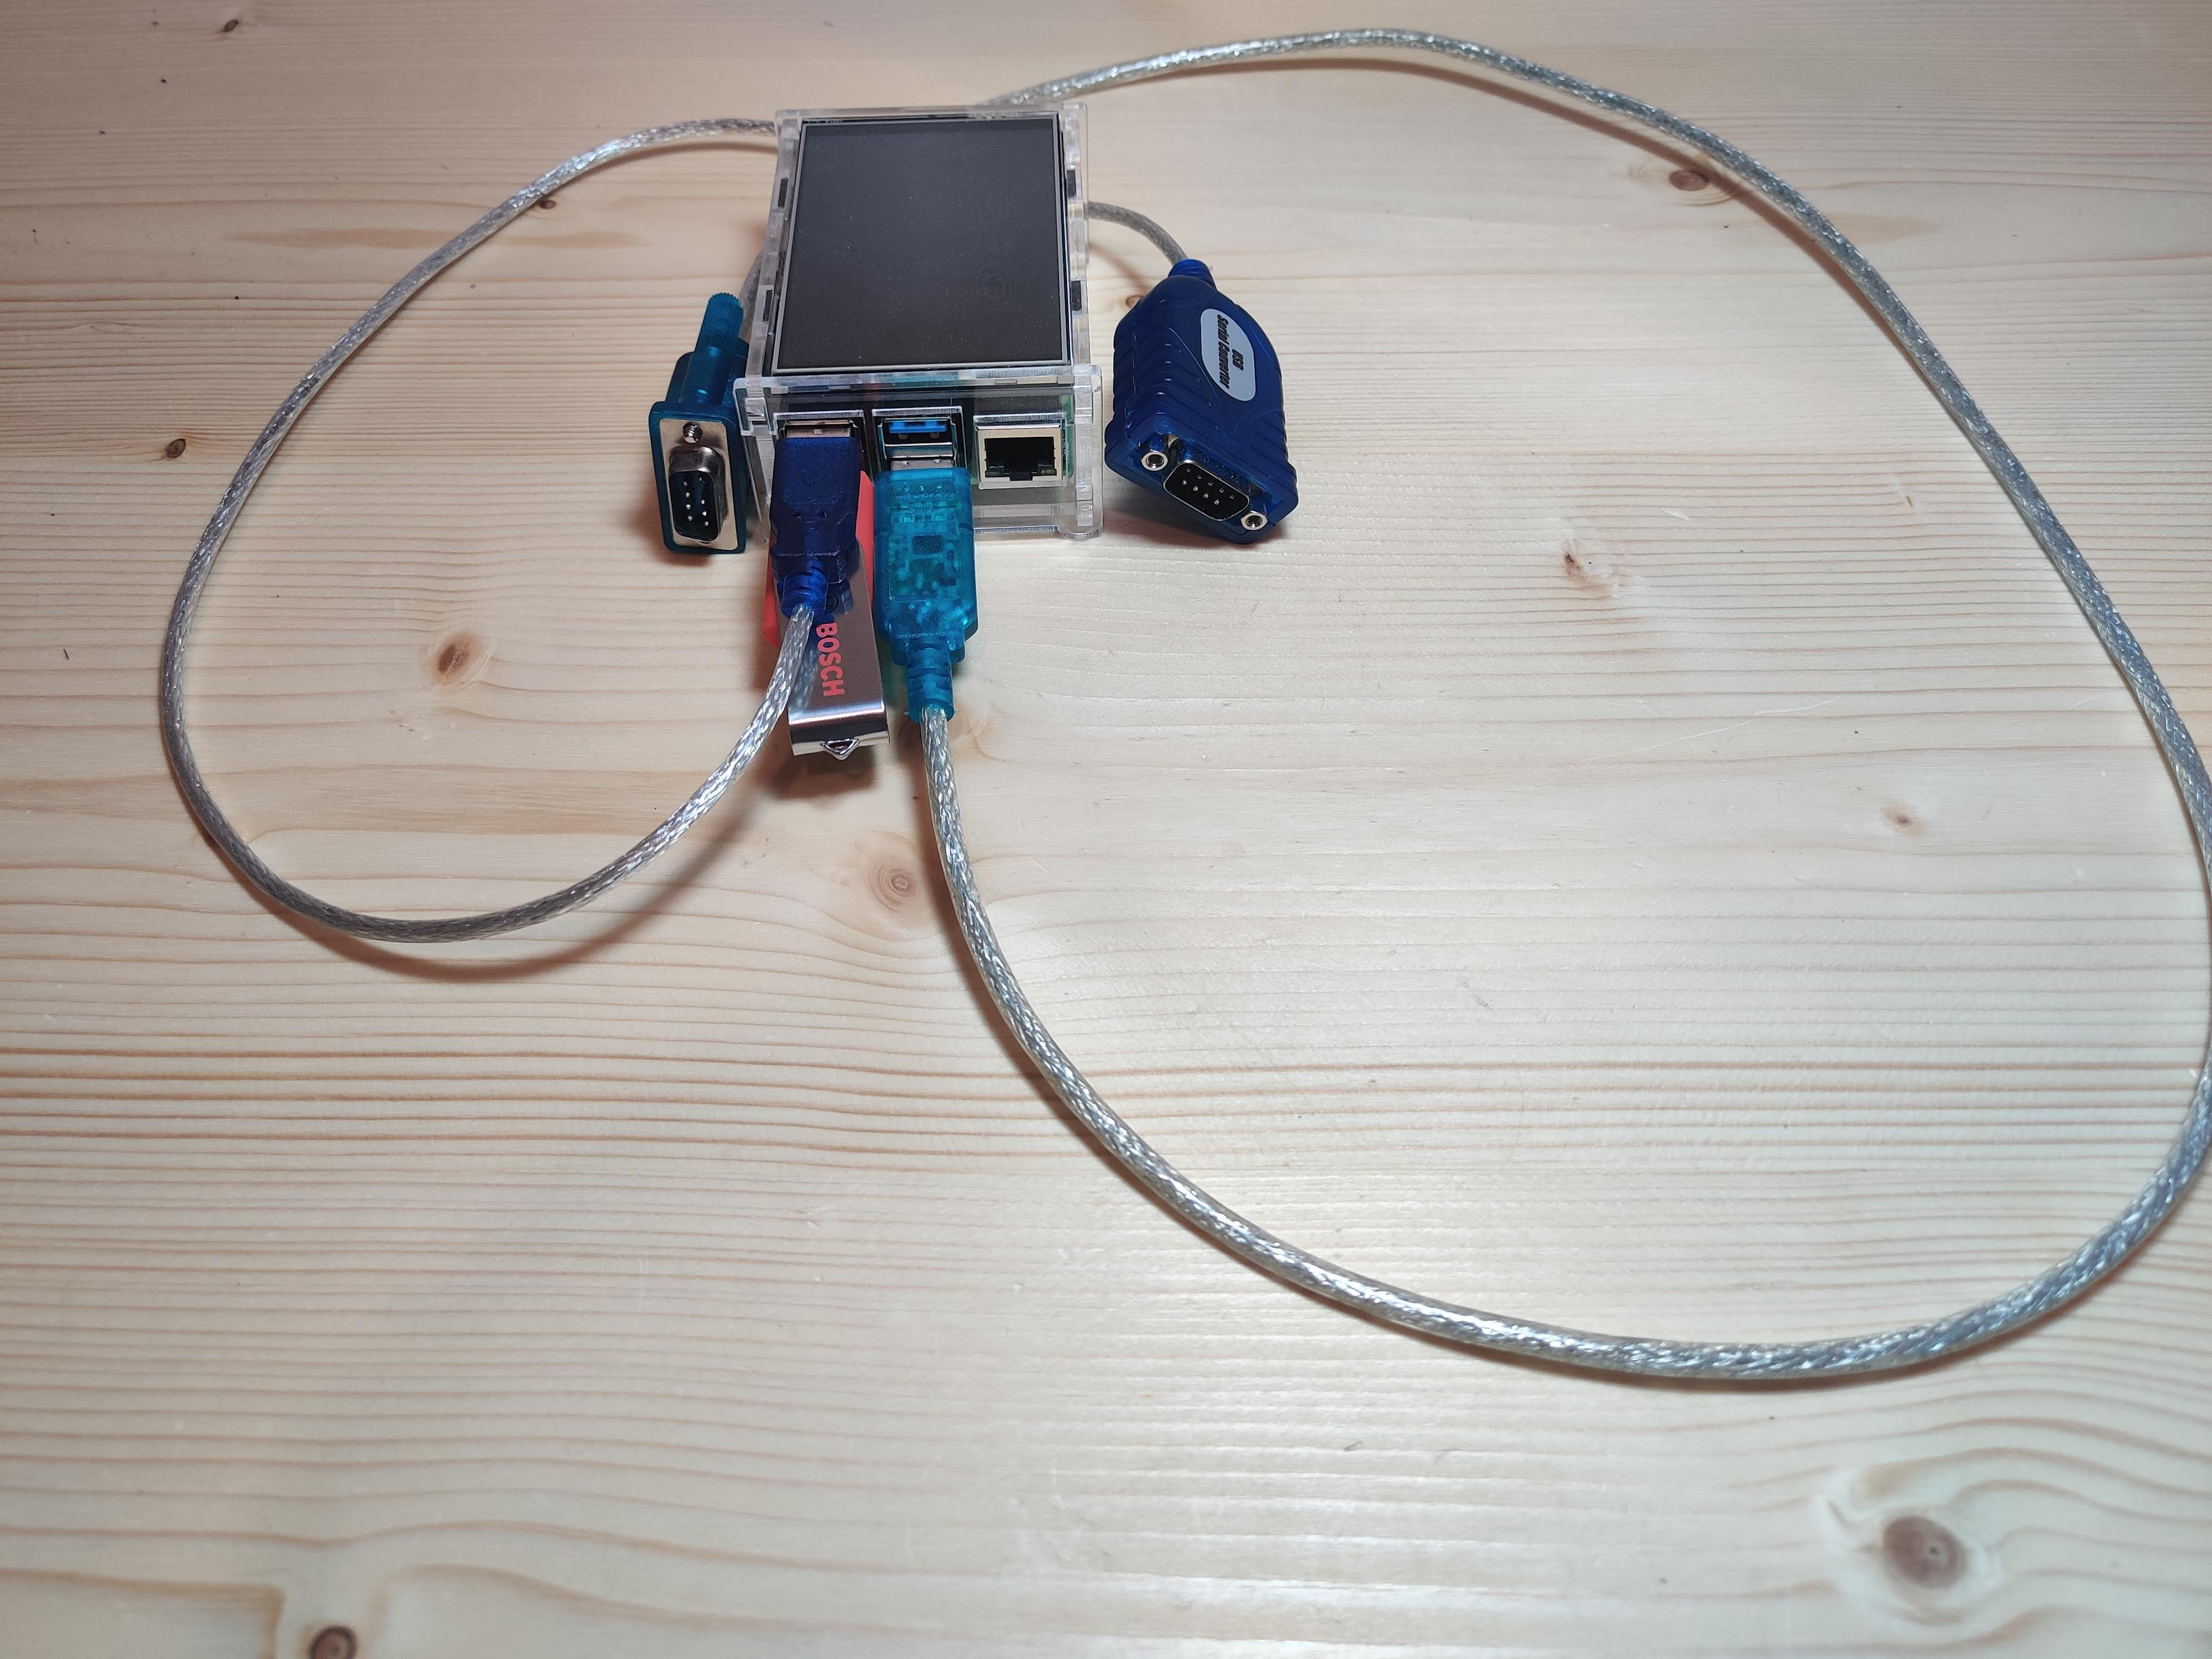
\includegraphics[width=1\textwidth]{hardware5.jpg}
\end{figure}
\section{Konfiguration}

\paragraph{}
Um eine serielle Schnittstelle auslesen zu können, müssen zuerst einige Parameter im Logging-Skript angepasst werden. Dazu gehören unter anderem, Speed(Baudrate), Anzahl der Datenbits, Anzahl der Stopbits und Parität der seriellen Schnittstelle. Diese Konfigurationen werden über SSH oder VNC vorgenommen. 

In beiden Fällen muss zuerst die IP-Adresse des eigenen Laptops auf eine IP-Adresse geändert werden, die im Subnet des RaspberryPi liegt und nicht mit anderen Adressen kollidiert.
\paragraph{IP des RaspberryPi}192.168.0.2/24
\paragraph{Freie IP-Adressen}192.168.0.3 - 192.168.0.254

\paragraph{Zugangsdaten}user: pi; passwort: 13571357

\pagebreak
\subsection{Anpassung des Logging-Skriptes an serielle Schnittstelle und Anwendungsfall}
\subsubsection{Möglichkeit 1: SSH}

\textbf{Für diese Variante sollten wissen, wie eine SSH-Verbindung aufgebaut wird. Außerdem wird ein Verständnis über die Bedienung von Linux per SSH-Terminal vorrausgesetzt. Erfüllen Sie diese Kriterien nicht fahren Sie bitte mit "Möglichkeit 2: VNC" fort.}

\begin{itemize}
	\item Die SSH Verbindung wird über den Standardport 22 und mit obiger IP hergestellt.
	\item Hierfür muss die Software Putty installiert werden. Putty liegt auf dem beiliegenden USB-Stick im Ordner Software/Putty.
	\item Verbinden Sie sich bitte mit dem Raspi. (user: pi; passwort: 13571357)
	\item Jetz muss ihr Anwendungssfall ausgewählt werden. 
	\item Zum Mitscheniden einer Output-Schnittstelle führen Sie bitte folgendes Kommando aus:
\begin{lstlisting}
cd /home/pi/Desktop/serial_logging/ && git stash && git checkout master  && cd /home/pi/Desktop/
\end{lstlisting}
\begin{lstlisting}
Moeglicher Output; beides ist OK:
1.
Switched to branch 'master'
Your branch is up to date with 'origin/master'.

2.
Already on 'master'
Your branch is up to date with 'origin/master'.
\end{lstlisting}
	\item Zum Mitscheniden einer Schnittstelle zwischen zwei Teilnehmern führen Sie bitte folgendes Kommando aus:
\begin{lstlisting}
cd /home/pi/Desktop/serial_logging/ && git stash && git checkout bidirectional  && cd /home/pi/Desktop/
\end{lstlisting}
\begin{lstlisting}
Moeglicher Output; beides ist OK:
1.
Switched to branch 'bidirectional'
Your branch is up to date with 'origin/bidirectional'.

2.
Already on 'bidirectional'
Your branch is up to date with 'origin/bidirectional'.
\end{lstlisting}
	
	\item Die Parameter der zu protokollierenden Schnittstelle werden direkt in das Skript eingetragen (Zeilen 11-19; siehe unten).
	\item Um das Skript zu bearbeiten stehen \textit{vim} und \textit{nano} zur Verfügung. 
	\item Siehe Anhang \ref{parameters} für alle möglichen Parameter.

\begin{lstlisting}
#/home/pi/Desktop/logging.py
#/home/pi/Desktop/logging_bidirectional.py
#Line 11-19

#=========================================================================== 
# Hier Parameter fuer die serielle Schnittstelle eintragen!!!
#=========================================================================== 
baudrate = 9600
parity = serial.PARITY_NONE
stopbits = serial.STOPBITS_ONE
bytesize = serial.EIGHTBITS
timeout = .1
#=========================================================================== 
\end{lstlisting}

	\item Das Skript muss als root mit python3 ausgeführt werden.
\begin{lstlisting}
sudo python3 /home/pi/Desktop/serial_logging/logging.py
\end{lstlisting}

\item Damit das Skript nicht mit dem Ende der SSH-Session beendet wird, kann \textit{screen} verwendet werden.
\end{itemize}


\begin{comment}
\FloatBarrier
\begin{figure}[h]
  \caption{Nur "Host Name (or IP address)" verändern!}
  \centering
    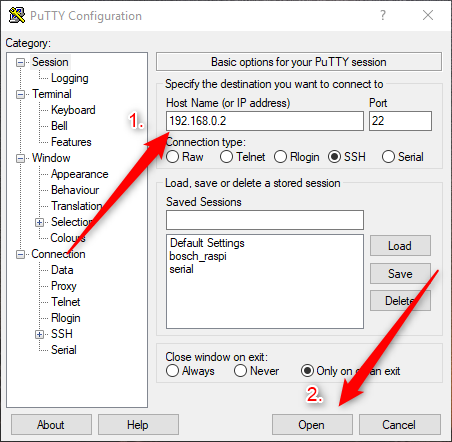
\includegraphics[height=0.5\textheight]{putty.png}
\end{figure}
\begin{figure}
  \caption{Benutzername "pi" eingeben und mit ENTER bestätigen.}
  \centering
    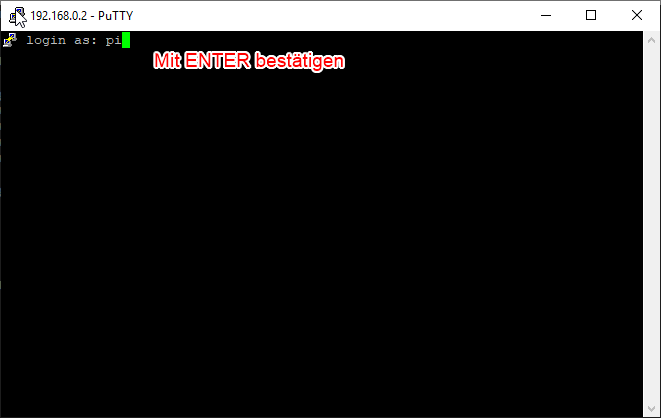
\includegraphics[height=0.4\textheight]{putty2.png}
\end{figure}
\begin{figure}
  \caption{Passwort "13571357" eingeben und mit ENTER bestätigen.
Achrung: Es sind keine Zeichen/Punkte/Sternchen sichtbar. Das ist normal!}
  \centering
    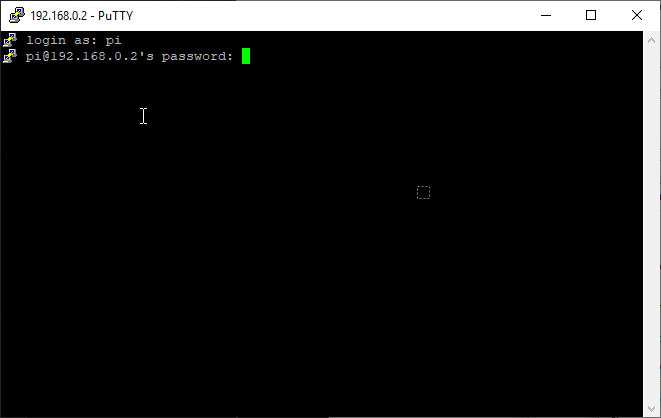
\includegraphics[height=0.4\textheight]{putty3.png}
\end{figure}
\end{comment}
\FloatBarrier




\FloatBarrier

\subsubsection{Möglichkeit 2: VNC mit grafischer Oberfläche}
\begin{itemize}
	\item Installation der Software VNC Viewer. VNC Viewer liegt auf dem beiliegenden USB-Stick im Ordnrer Software/vnc\_viewer.
	\item Starten Sie bitte nun den VNC Viewer.
	\item Um nun die Verbindung zum RaspberryPi herzustellen, folgen Sie bitte den Anweisungen der Screenshots auf den nächsten Seiten.
\begin{figure}[h]
  \caption{IP-Adresse eingeben und mit Enter bestätigen. Nicht rechts auf Anmelden!}
  \centering
    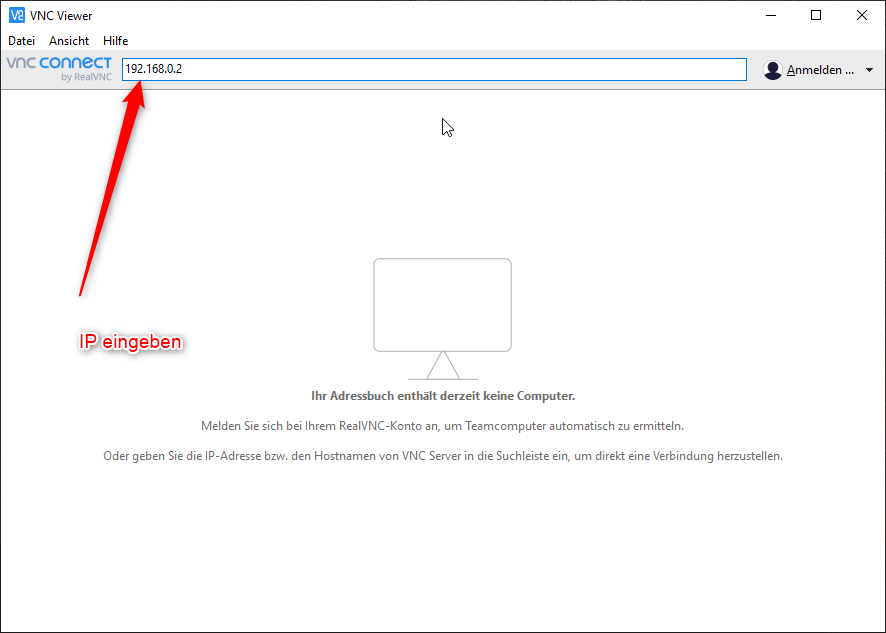
\includegraphics[width=1\textwidth]{vnc.png}
\end{figure}
\begin{figure}
  \caption{Als Benutzer "pi" eingeben; als Passwort "13571357" eingeben; mit ENTER bestätigen.}
  \centering
    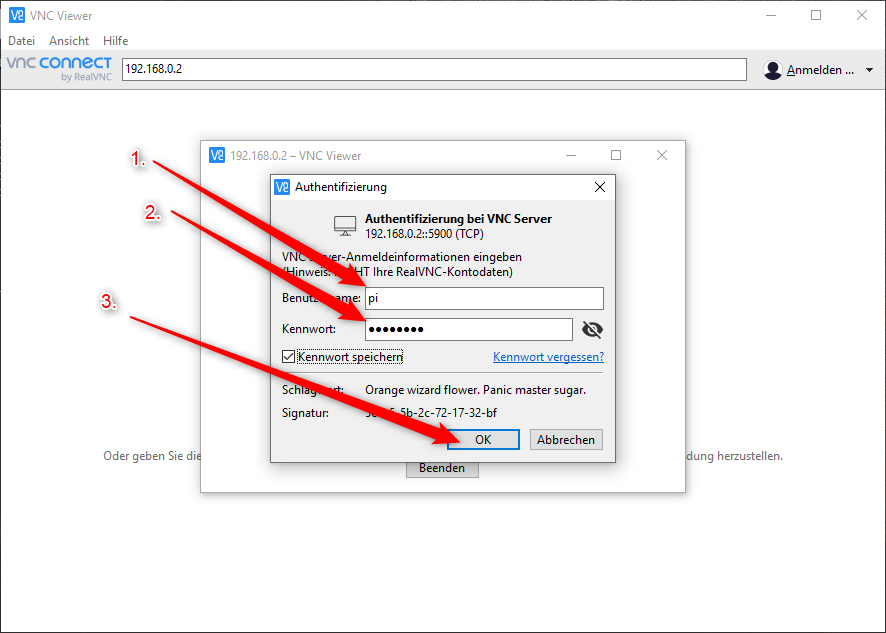
\includegraphics[width=1\textwidth]{vnc2.png}
\end{figure}
\begin{figure}
  \caption{Bei erfolgreicher Verbindung erscheint der Desktop.}
  \centering
    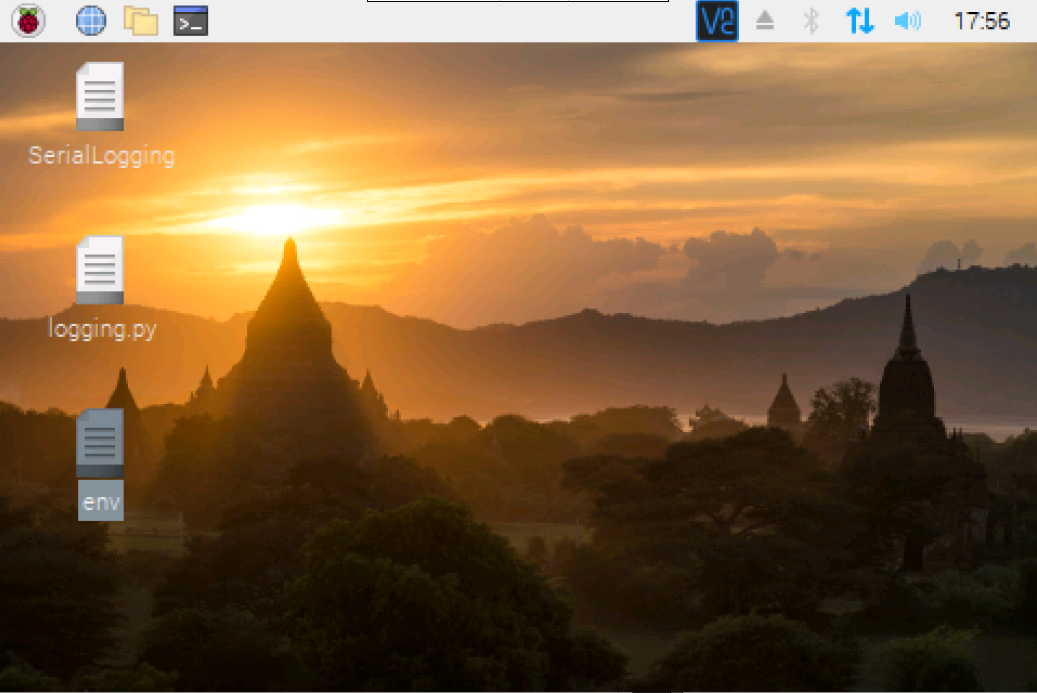
\includegraphics[width=1\textwidth]{vnc3.png}
\end{figure}
\FloatBarrier

	\item Jetz muss ihr Anwendungssfall ausgewählt werden. 
	\item Öffnen Sie bitte ein Terminal mit STRG+ALT+T
	\item Zum Mitscheniden einer Output-Schnittstelle führen Sie bitte folgendes Kommando aus:
\begin{lstlisting}
cd /home/pi/Desktop/serial_logging/ && git stash && git checkout master  && cd /home/pi/Desktop/
\end{lstlisting}
\begin{lstlisting}
Moeglicher Output; beides ist OK:
1.
Switched to branch 'master'
Your branch is up to date with 'origin/master'.

2.
Already on 'master'
Your branch is up to date with 'origin/master'.
\end{lstlisting}
	\item Zum Mitscheniden einer Schnittstelle zwischen zwei Teilnehmern führen Sie bitte folgendes Kommando aus:
\begin{lstlisting}
\textsc{cd /home/pi/Desktop/serial_logging/ && git stash && git checkout bidirectional  && cd /home/pi/Desktop/}
\end{lstlisting}
\begin{lstlisting}
Moeglicher Output; beides ist OK:
1.
Switched to branch 'bidirectional'
Your branch is up to date with 'origin/bidirectional'.

2.
Already on 'bidirectional'
Your branch is up to date with 'origin/bidirectional'.
\end{lstlisting}
	\item Das Terminal kann nun wieder geschlossen werden.
	\item Die Parameter der zu protokollierenden Schnittstelle werden direkt in das Skript eingetragen (Zeile 11-19).
	\item Wechseln Sie in den Ordner serial\_logging auf dem Desktop
	\item Rechtsklick auf die Datei logging.py
	\item Änderungen Durchführen wie unten beschrieben. Siehe Anhang \ref{parameters} für alle möglichen Parameter.
	\item Editor mit "X" beenden
	\item Änderungen mit "save" übernehmen
	\item Dateiexplorer mit "X" beenden
\end{itemize}

\begin{lstlisting}
#/home/pi/Desktop/logging.py
#/home/pi/Desktop/logging_bidirectional.py
#Line 11-19

#=========================================================================== 
# Hier Parameter fuer die serielle Schnittstelle eintragen!!!
#=========================================================================== 
baudrate = 9600
parity = serial.PARITY_NONE
stopbits = serial.STOPBITS_ONE
bytesize = serial.EIGHTBITS
timeout = .1
#=========================================================================== 
\end{lstlisting}


\section{Ausführen des Logging-Skriptes}
\paragraph{VNC}
\begin{itemize}
	\item Doppelklick auf SerialLogging auf dem Desktop
	\item "Execute" im sich öffnenden Fenster.
\end{itemize}

\paragraph{SSH}
\begin{itemize}
	\item Das Skript wird bei normaler Ausführung bei Beendigung der SSH-Session terminiert.
	\item Um das Skript weiterlaufen zu lassen, kann z.B. Screen verwendet werden.
\end{itemize}

\begin{lstlisting}
screen \textsc{sudo python3 /home/pi/Desktop/serial_logging/logging.py}

Detach
To detach this terminal session, press
CTRL + A     release, and then press   D
Then you are back in the original terminal screen with the other one running detached in the background.

List all Instances
You can list all open screen instances and their status by typing...
screen -list

Reconnect
...and you can reconnect to an instance with...
screen -r

If you only have one screen instance open, just -r will be enough. If you have more than one, you have to specify which one you want to reconnect with by typing its name after the -r
\end{lstlisting}




\section{Anhang}
\subsection{Parameter für serielle Schnittstellen} \label{parameters}

\paragraph{Standardparameter} 
\begin{itemize}
    \item baudrate (int): Baud rate such as 9600 or 115200 etc.
    \item bytesize: Number of data bits. Possible values: FIVEBITS, SIXBITS, SEVENBITS, EIGHTBITS
    \item parity: Enable parity checking. Possible values: PARITY\_NONE, PARITY\_EVEN, PARITY\_ODD PARITY\_MARK, PARITY\_SPACE
    \item stopbits: Number of stop bits. Possible values: STOPBITS\_ONE, STOPBITS\_ONE\_POINT\_FIVE, STOPBITS\_TWO
\end{itemize}

\paragraph{Weitere Parameter (nur über direkten Eintrag ins Skript)} 
\begin{itemize}
	\item timeout (float): Set a read timeout value.
    \item xonxoff (bool): Enable software flow control.
    \item rtscts (bool): Enable hardware (RTS/CTS) flow control.
    \item dsrdtr (bool): Enable hardware (DSR/DTR) flow control.
    \item write\_timeout (float): Set a write timeout value.
    \item inter\_byte\_timeout (float): Inter-character timeout, None to disable (default).
    \item exclusive (bool): Set exclusive access mode (POSIX only). A port cannot be opened in exclusive access mode if it is already open in exclusive access mode.
\end{itemize}

\subsection{Dateien auf USB-Stick}
\begin{lstlisting}
Software
	|-Putty
	|-VNC Viewer
Sonstiges
	|-baseimage --> Herstellerimage mit Displaytreiber
	|-documentation --> LATEX-Version der Dokumentation
documentation.pdf
serial_logging_final --> Image mit Loggingskript
\end{lstlisting}

\end{document}
